%!TEX root = draft.tex
\section{Application to the Stefan problem} \label{sec:application}

\subsection{Presentation of the problem}

In this section we apply our approach to the study of the phase transition of a liquid melt to a solid crystaline structure. In the case of a single component melt, and in the absence of convection, the process is dominated by diffusion and can be modeled as a Stefan problem. We decompose the computational domain $\Omega$ into two subdomains $\Omega_l$ and $\Omega_s$, separated by an interface $\Gamma$. The Stefan problem describes the evolution of the temperature $T$, decomposed into $T_s$ in the solid phase $\Omega_s$ and $T_l$ in the liquid phase $\Omega_l$, as
\begin{align}
\pd{T_l}{t} & = D_l \Delta T_l \quad \mathrm{in} ~~ \Omega_l, \label{eq:stefan_heat_equation_l} \\
\pd{T_s}{t} & = D_s \Delta T_s \quad \mathrm{in} ~~ \Omega_s. \label{eq:stefan_heat_equation_s}
\end{align}
The diffusion constants $D_l$ and $D_s$ can be discontinuous across the interface. We prescribe homogeneous Neumann boundary conditions on the edge of the computational domain, $\nabla T \cdot \underline{\mathbf{n}}\vert_{\partial \Omega}=0$. At the interface between the solid and the liquid phases, the temperature is given by the Gibbs-Tompson boundary condition \cite{Alexiades;Solomon;Wilson:88:The-formation-of-a-s, Alexiades;Solomon:93:Mathematical-Modelin}:
\begin{equation} \label{eq:stefan_gibbs_tompson}
T_s = T_l = T_{\Gamma} = -\epsilon_c \kappa - \epsilon_v (\underline{\mathbf{u}} \cdot \underline{\mathbf{n}}),
\end{equation}
where $\kappa$ is the local interface curvature, $\underline{\mbf{u}}$ is the velocity of the interface, $\underline{\mathbf{n}}$ is the outward normal to the solidification front and $\epsilon_c$ and $\epsilon_v$ are the surface tension and kinetic undercooling coefficients. The interface velocity $\underline{\mbf{u}}$ is defined from the jump in the heat flux at the interface,
\begin{equation} \label{eq:stefan_velocity}
(\underline{\mathbf{u}} \cdot \underline{\mathbf{n}}) = - \left[ D_l \pd{T_l}{\underline{\mathbf{n}}} - D_s \pd{T_s}{\underline{\mathbf{n}}} \right].
\end{equation}
We choose to use an adaptive time step with a $\text{CFL} = 5$, i.e.
\begin{equation} \label{eq:stefan_dt}
\Delta t = 5 ~ \Delta x_{min} ~ \min(1,1/\max \lVert \underline{\mathbf{u}} \rVert),
\end{equation}
where $\Delta x_{min}$ is the size of the smallest cell of the forest. The general procedure to solve the Stefan problem is presented in Algorithm \ref{alg:stefan} and we refer the interested reader to \cite{Chen;Min;Gibou:09:A-numerical-scheme-f} for the details of implementation. In implementing the numerical solver, we make use of the popular \texttt{PETSc}
\cite{Balay;Abhyankar;Adams;etal:14:PETSc-Web-page} library for linear algebra and its parallel primitives, such as parallel ghosted vector and scatter/gather operations, which simplifies the implementation.


\begin{algorithm}[htbp]
\caption{$\texttt{General procedure for solving the Stefan problem}$}
\begin{algorithmic}[1]
\State Initialize the forest and $\phi$ given the initial geometry.
\State Initialize $T_s$ in $\Omega^+$ and $T_l$ in $\Omega^-$.
\State Reinitialize $\phi$ and compute the local interface curvature $\kappa$.
\State Compute $T^{n+1}_l$ and $T^{n+1}_s$ by solving the heat equations \eqref{eq:stefan_heat_equation_l} and \eqref{eq:stefan_heat_equation_s}.
\State Extrapolate $T^{n+1}_s$ from $\Omega^+$ to $\Omega^-$ and $T^{n+1}_l$ from $\Omega^-$ to $\Omega^+$.
\State Compute the velocity field $\underline{\mathbf{u}}$ according to \eqref{eq:stefan_velocity}.
\State Compute the time step dt following \eqref{eq:stefan_dt}.
\State Evolve the interface and construct the new forest using the Semi-Lagrangian procedure.
\State Interpolate $T^{n+1}_s$ and $T^{n+1}_l$ from the old forest to the new forest.
\State Go to 3 with n=n+1.
\end{algorithmic}
\label{alg:stefan}
\end{algorithm}

\subsection{Scalability}

The implementation of the Stefan problem relies on the components described in the previous sections, and it is therefore a good synthesis of the performance of the various algorithms. We monitored the performance of the code over five time iterations, as presented in Algorithm \ref{alg:stefan}, for two different maximum resolutions. In both cases, the forest is built on a $20\times20\times20$ macro-mesh. The maximum tree resolution for the small test is 9, leading to approximately 7M grid points, and the maximum resolution for the large test is 11, corresponding to 105M grid points. The level-set function is reinitialized at every time-step by applying 20 iterations of the reinitialization procedure. The results are presented in figure \ref{fig:stefan_scaling}, where ``\verb|Solution_Extension|'' refers to extrapolation procedure (see Algorithm \ref{alg:stefan} step 5). As expected from the results obtained for each component in the previous sections, our implementation of the Stefan problem exhibits very satisfactory scaling (cf.\ Table \ref{tab:scaling_stefan}).

\begin{figure}
\centering
\subfigure[]{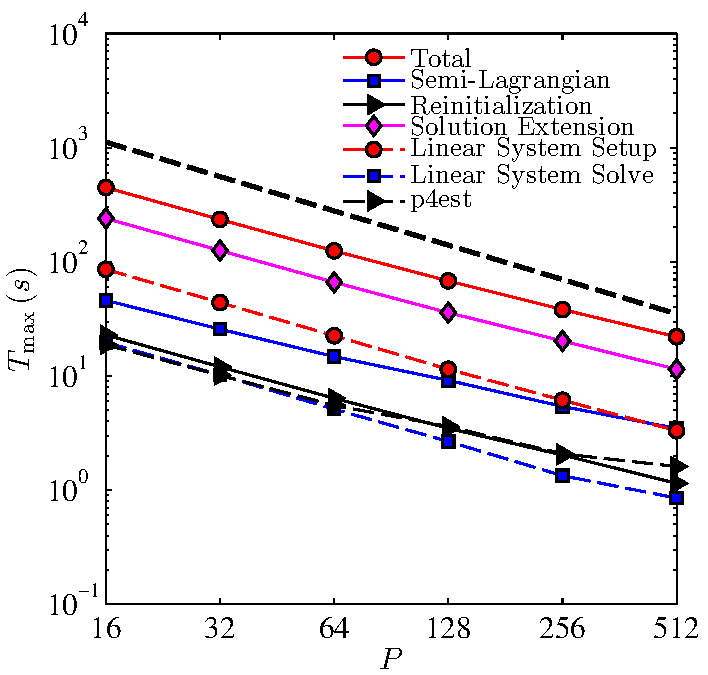
\includegraphics[width=0.48\textwidth]{figures/Stefan_small.pdf}}
\subfigure[]{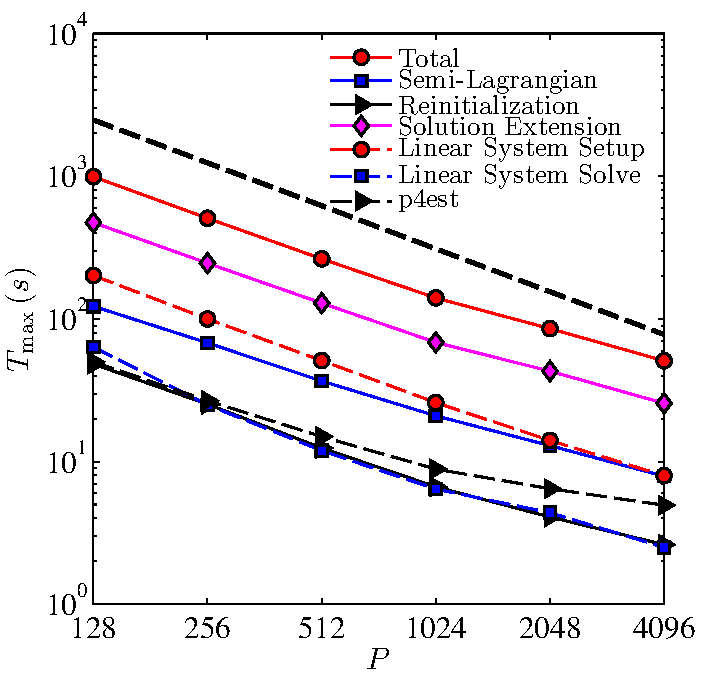
\includegraphics[width=0.48\textwidth]{figures/Stefan_large.pdf}}
\caption{Scalability of the Stefan problem for small (left) and large (right) Octrees with roughly 7M and 105M grid points, respectively. The solid dashed line represents perfect scaling. As expected from the scalability analysis of the individual components, we observe excellent results, illustrating the potential of our algorithms.}
\label{fig:stefan_scaling}
\end{figure}

\begin{table}
\centering
	\begin{tabular}{|l|c|cccccc|}
	\hline
	\multirow{2}{*}{Small Test} & $P$ & 16      & 32      & 64      & 128     & 256    & 512 \\ 	                            
	                            & $e$ & $100\%$ & $95\%$  & $90\%$  & $82\%$  & $73\%$ & $64\%$ \\
	\hline
	\multirow{2}{*}{Large Test} & $P$ & 128     & 256     & 512     & 1024    & 2048   & 4096 \\ 	                            
	                            & $e$ & $100\%$ & $98\%$  & $94\%$  & $89\%$  & $73\%$ & $61\%$ \\
	\hline
	\end{tabular}
	\caption{Parallel efficiency of the total runtime for the Stefan test based on the lowest number of processes for each test.}
	\label{tab:scaling_stefan} 
\end{table}

\subsection{Numerical experiments}
We now present the results from a large simulation of the Stefan problem on a $20\times20\times20$ macro-mesh and with level-10 Octrees. The Gibbs-Tompson anisotropy undercooling coefficients in equation \eqref{eq:stefan_gibbs_tompson} are defined as
\begin{align*}
\epsilon_c & = \left[ \epsilon_1 \left( 1+\alpha_1 \cos(3\theta_1) \right) + \epsilon_2 \left( 1+\alpha_2 \cos(3\theta_2) \right) \right] \kappa,\\
\epsilon_v & = 0,
\end{align*}
with $\theta_1$ the angle between the normal to the interface $\underline{\mathbf{n}}$ and the x-axis in the $(x,y)$ plane and $\theta_2$ the angle between $\underline{\mathbf{n}}$ and the x-axis in the $(x,z)$ plane. The coefficients
\begin{align*}
\epsilon_1 & = 2~(\sin(x)+\cos(y)+2)\cdot10^{-6}, & \epsilon_2 & = 2~(\sin(x)+\cos(z)+2)\cdot10^{-6}, \\
\alpha_1 & = \frac{1}{4}(\cos(x)+\sin(y)+2), & \alpha_2 & = \frac{1}{4}(\cos(x)+\sin(z)+2),
\end{align*}
are used to enforce a variety of crystal shapes. The computation is initialized with twenty spherical seeds of radius $1.5 \cdot 10^{-3}$ placed randomly in the domain. We take the diffusion coefficients $D_s=D_l=1$ and set the initial temperatures $T^0_l=-0.25$ and $T^0_s=0$.

The simulation was ran on $256$ MPI processes for $6$ hours and $30$ minutes, resulting in $396$ time iterations. Visualizations of the final iteration are presented in figures \ref{fig:stefan_grid} and \ref{fig:stefan_evolution}. The final iteration of the simulation consisted of $167$M grid points whereas a uniform grid with the equivalent finest resolution would lead to $8.59\cdot10^{12}$ grid points, i.e. over eight trillion grid points. Our simulation used only $0.002\%$ of the number of grid points needed for the same simulation on a uniform grid. This application demonstrates the ability of our approach to resolve small scale details, while accounting for long range interactions.

\begin{figure}[ht!]
\begin{center}
\subfigure[]{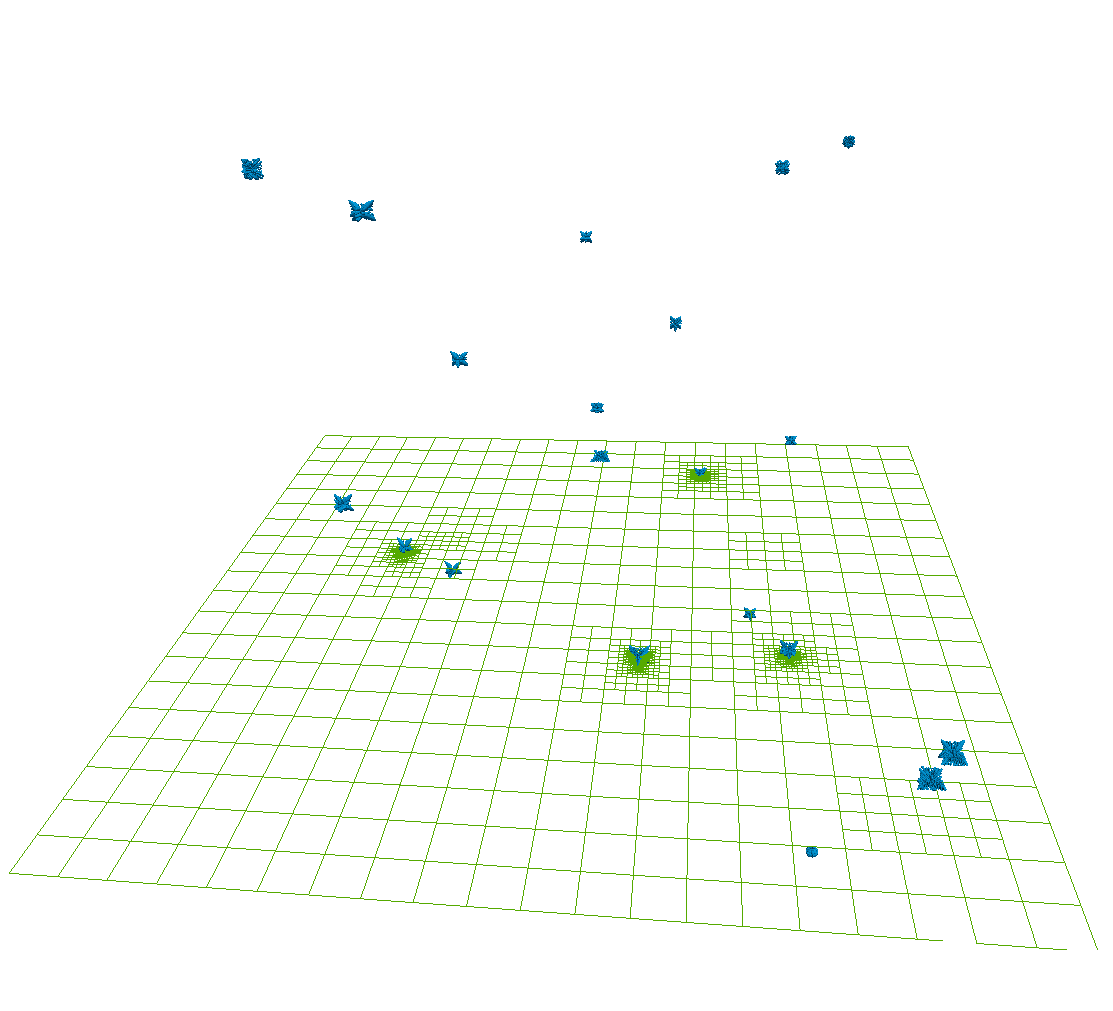
\includegraphics[width=0.45\textwidth]{figures/stefan_grid_overview.png}}
\subfigure[]{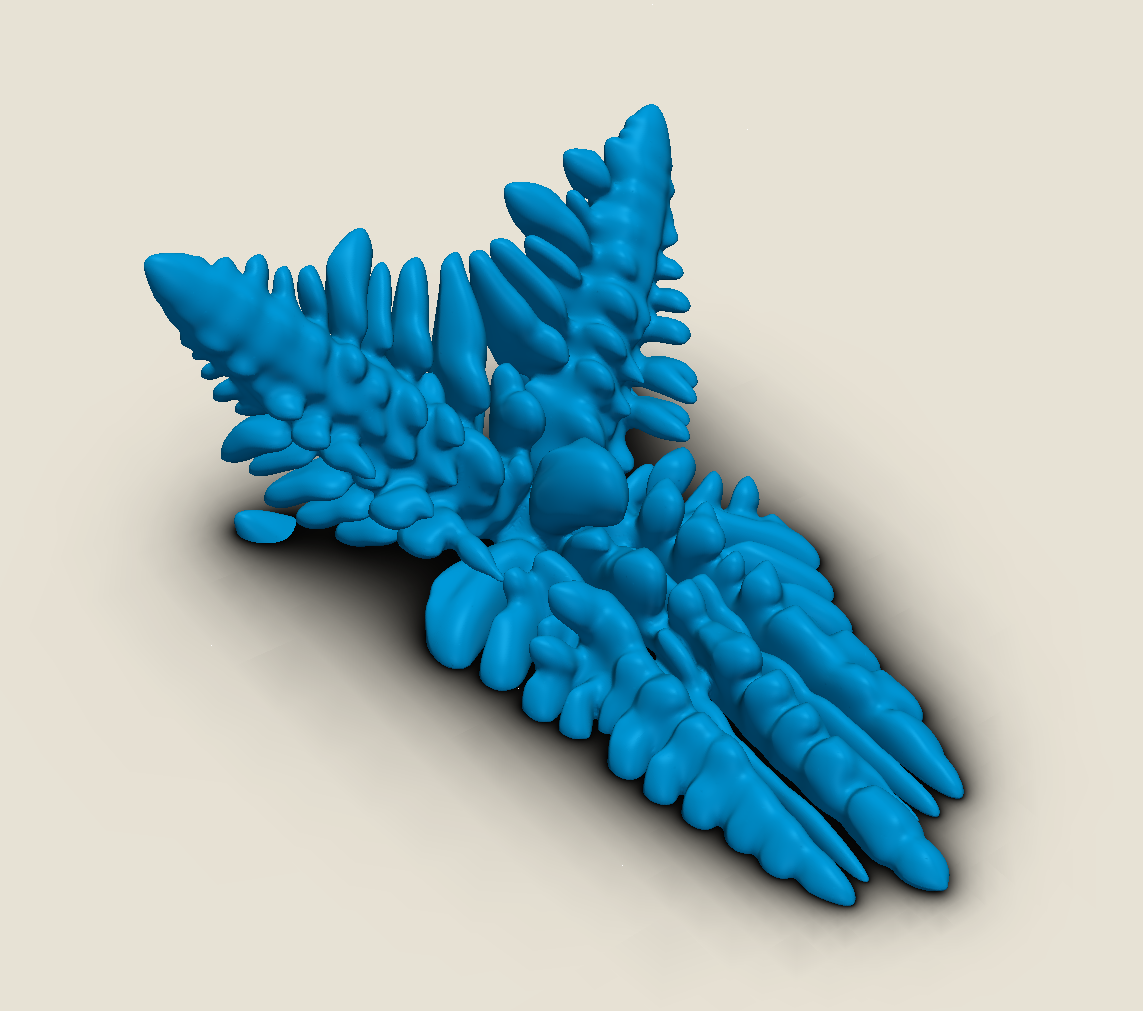
\includegraphics[width=0.45\textwidth]{figures/stefan_temperature.png}}
\subfigure[]{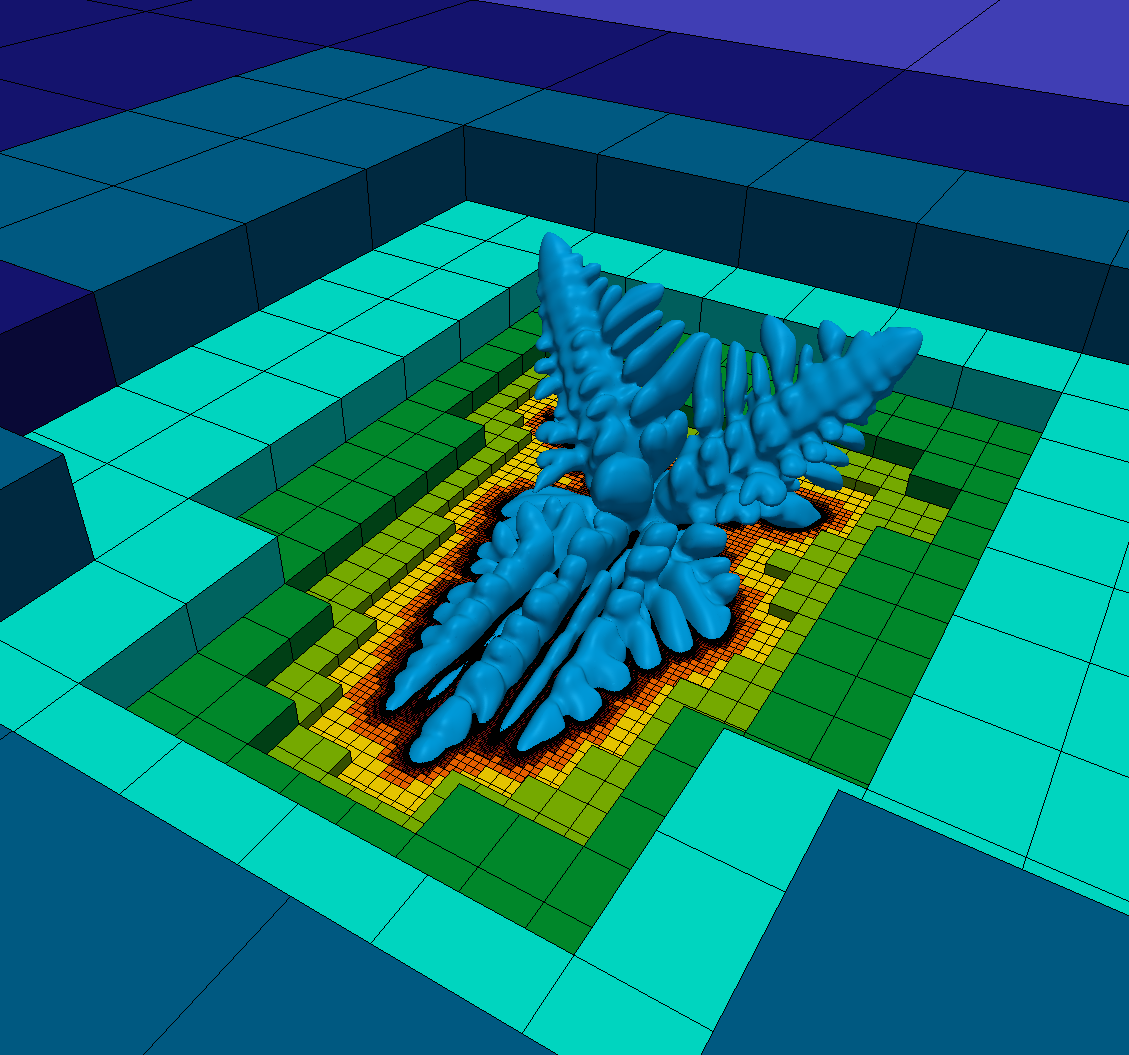
\includegraphics[width=0.45\textwidth]{figures/stefan_grid.png}}
\subfigure[]{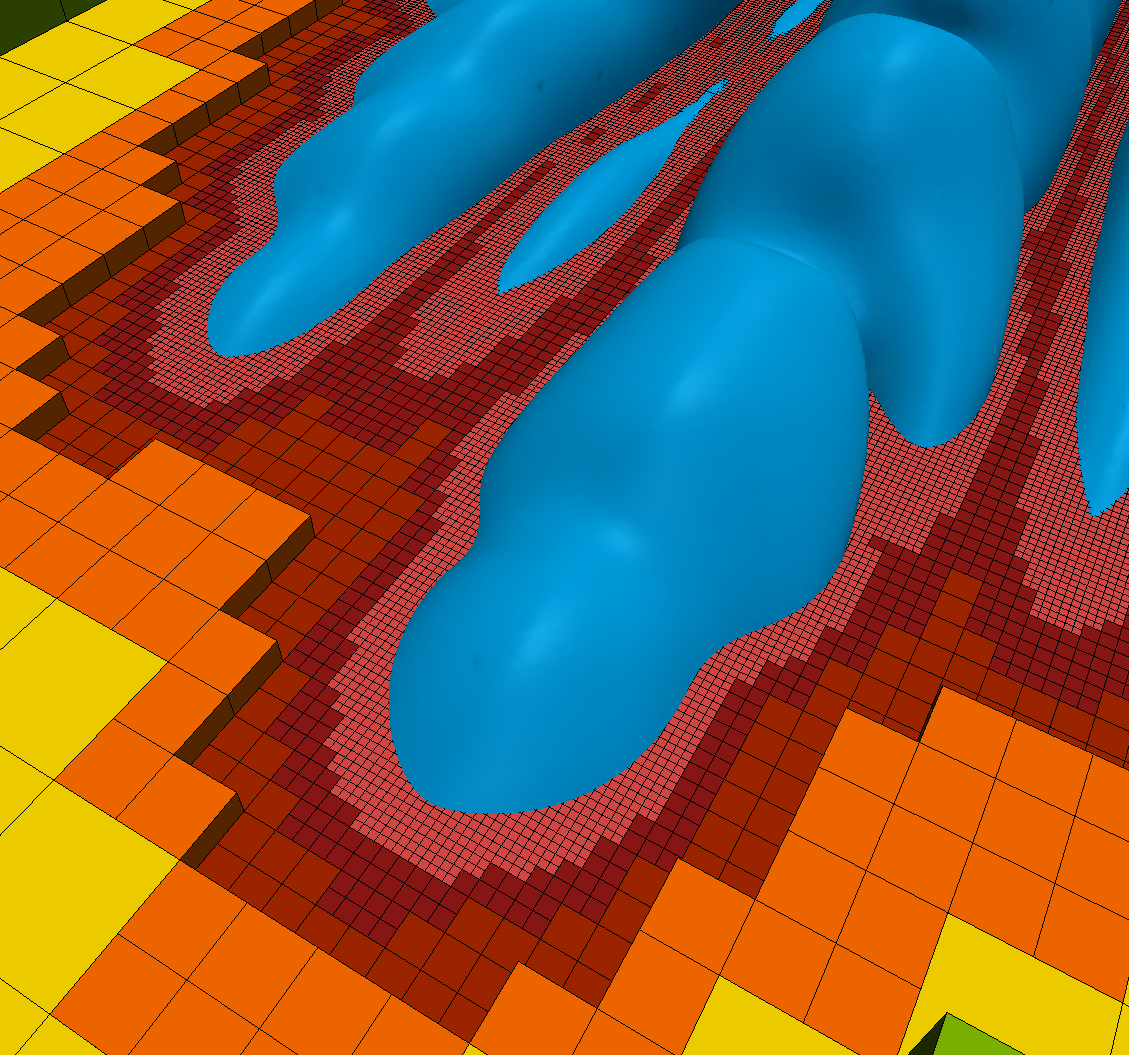
\includegraphics[width=0.45\textwidth]{figures/stefan_grid_zoom.png}}
\caption{Visualization of the computational mesh (a, c, d) and the temperature field (b) for the Stefan problem simulation.} \label{fig:stefan_grid}
\end{center}
\end{figure}

%\begin{figure}[ht!]
%\begin{center}
%\subfigure[]{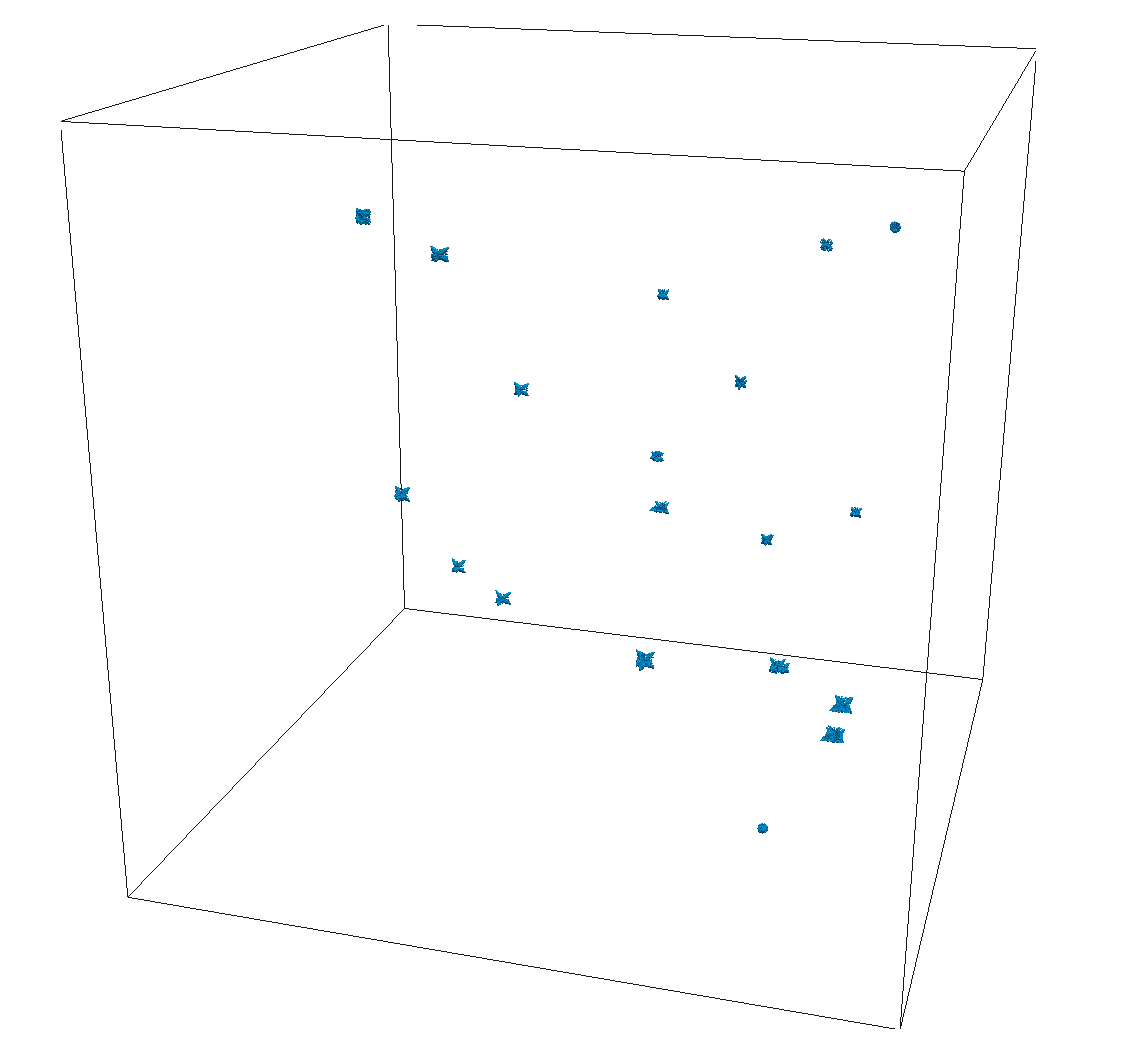
\includegraphics[width=0.45\textwidth]{figures/stefan_crystal_1.png}}
%\subfigure[]{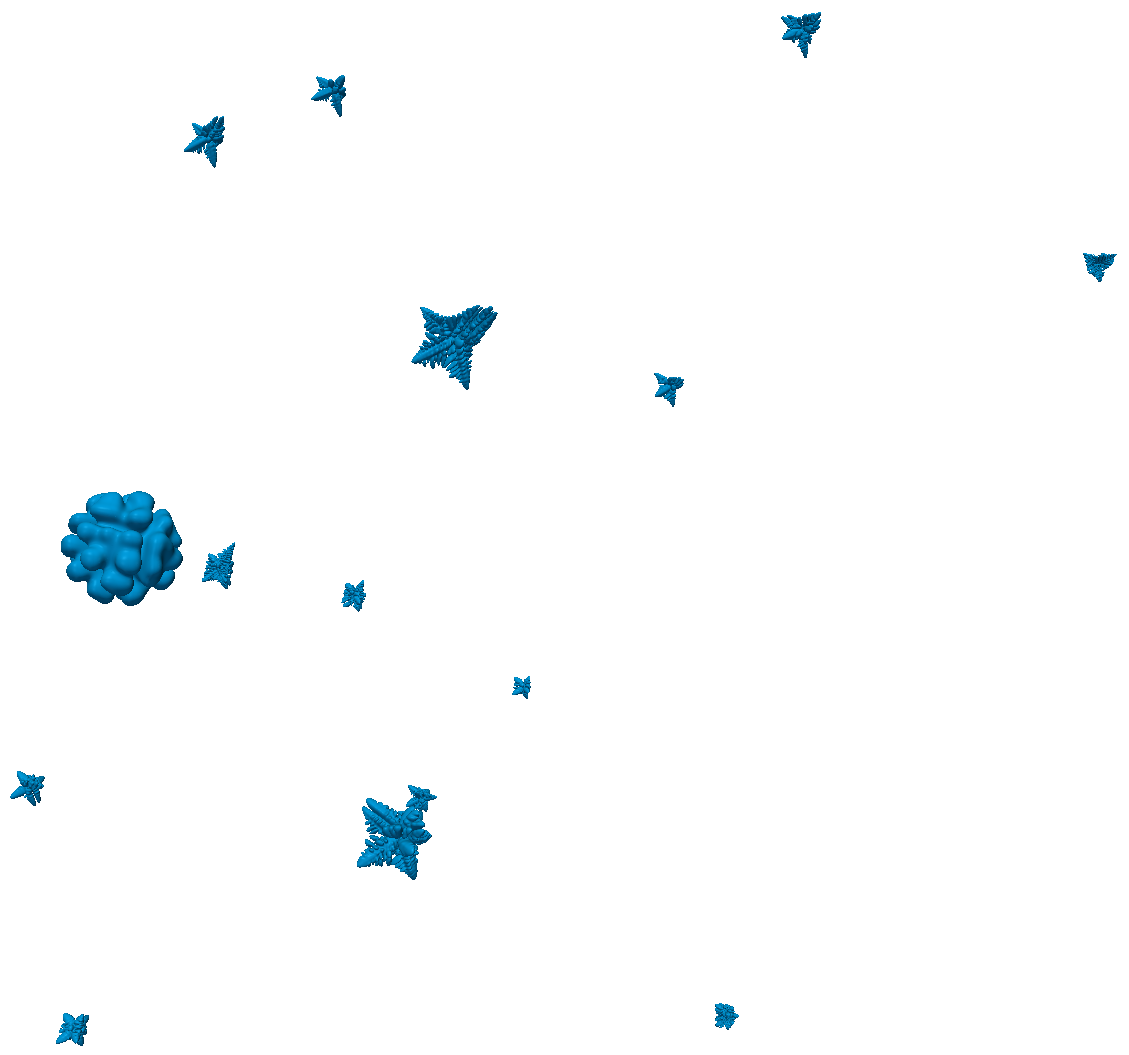
\includegraphics[width=0.45\textwidth]{figures/stefan_crystal_2.png}}
%\subfigure[]{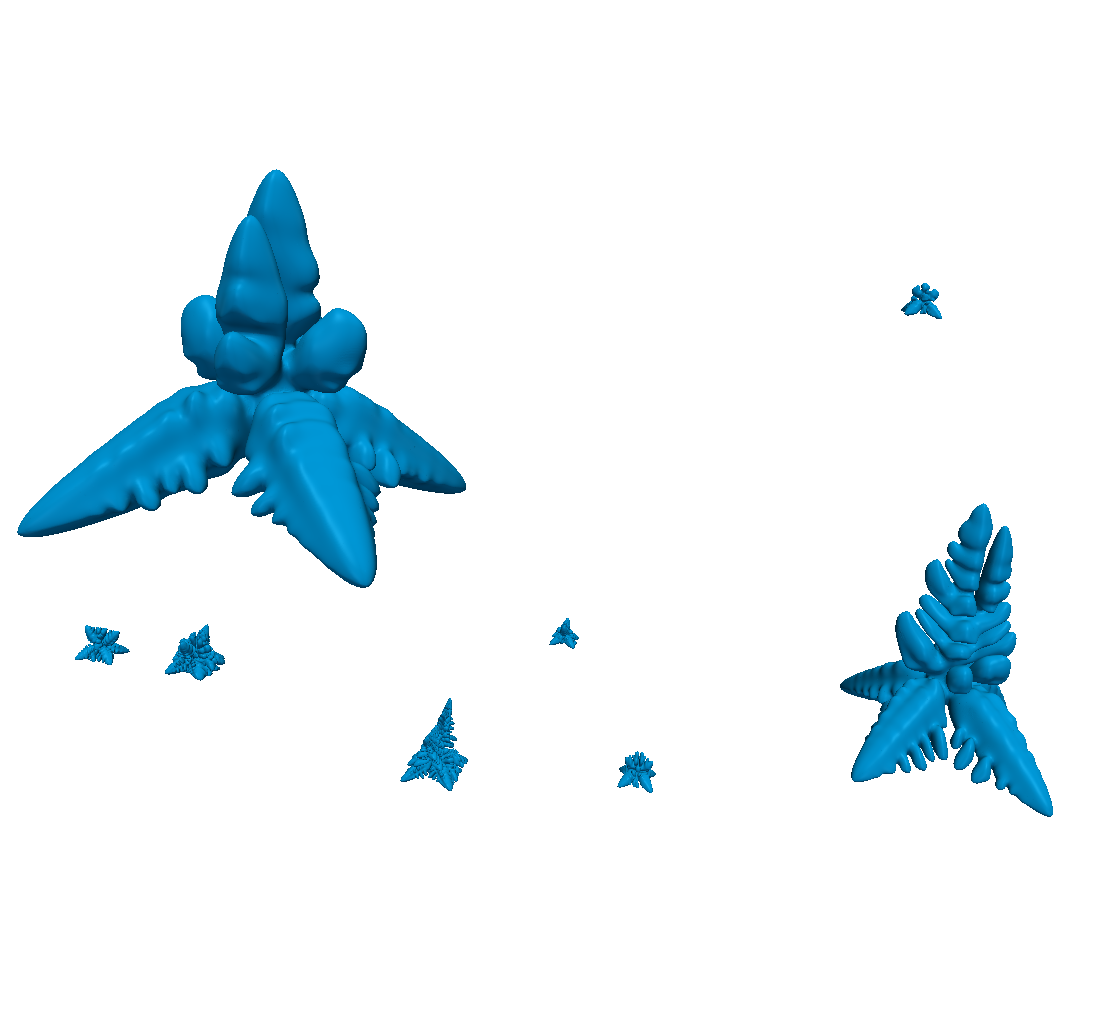
\includegraphics[width=0.45\textwidth]{figures/stefan_crystal_4.png}}
%\subfigure[]{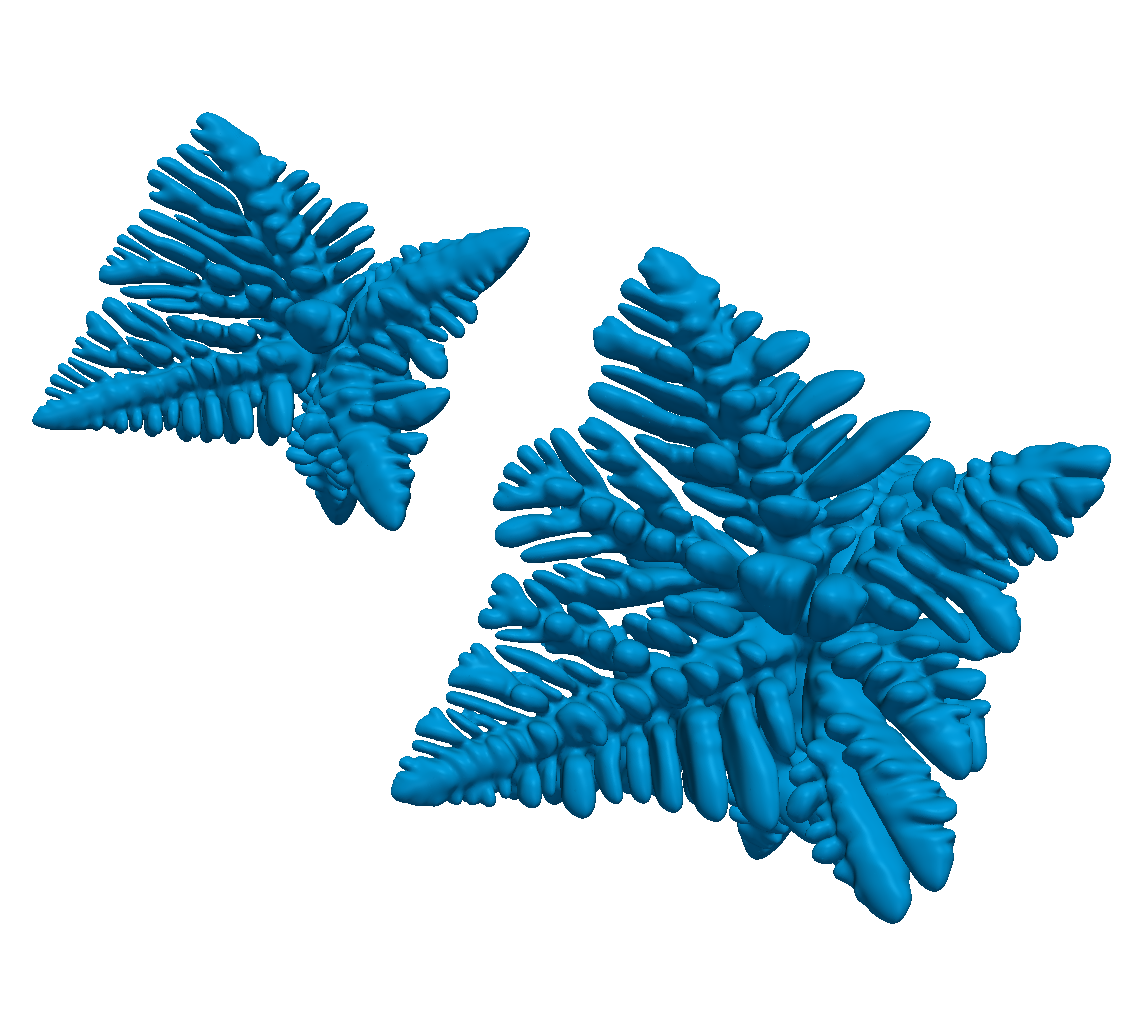
\includegraphics[width=0.45\textwidth]{figures/stefan_crystal_3.png}}
%\caption{Representation of the computational domain (a) as well as various developped crystal structures obtained from solving the Stefan problem simulation (b,c,d).} \label{fig:stefan_crystals}
%\end{center}
%\end{figure}

\begin{figure}[ht!]
\begin{center}
\subfigure{
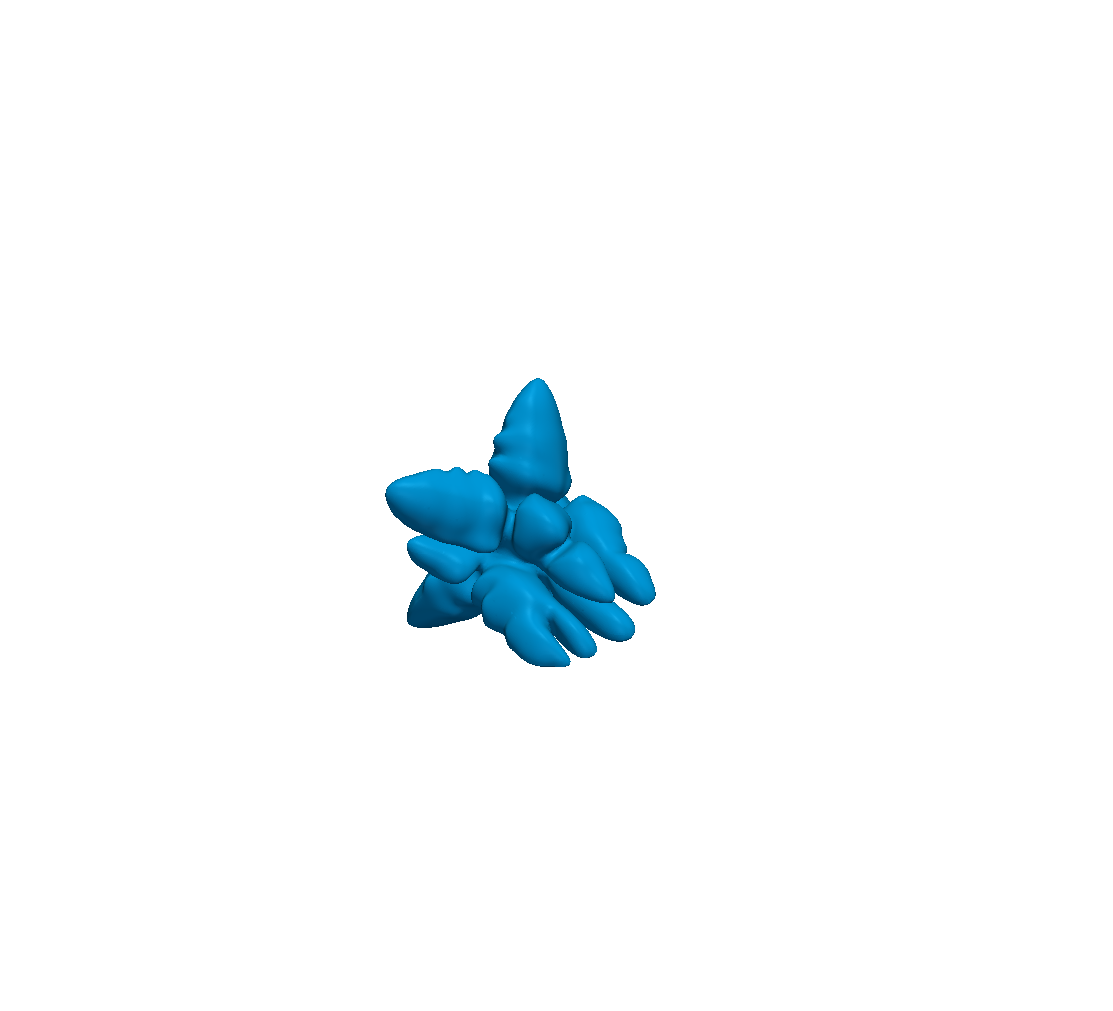
\includegraphics[width=.24\textwidth]{stefan/nb2_iter19.png}
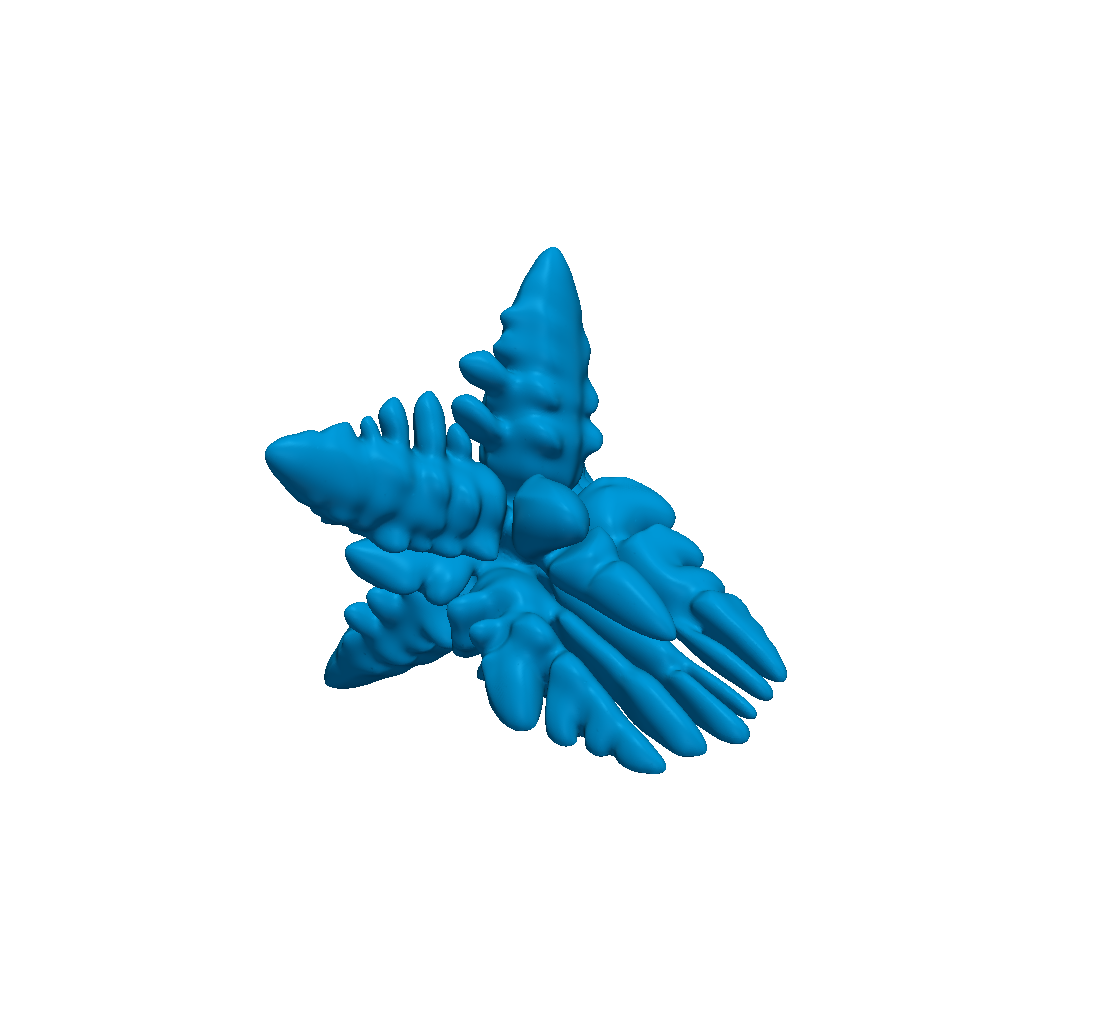
\includegraphics[width=.24\textwidth]{stefan/nb2_iter39.png}
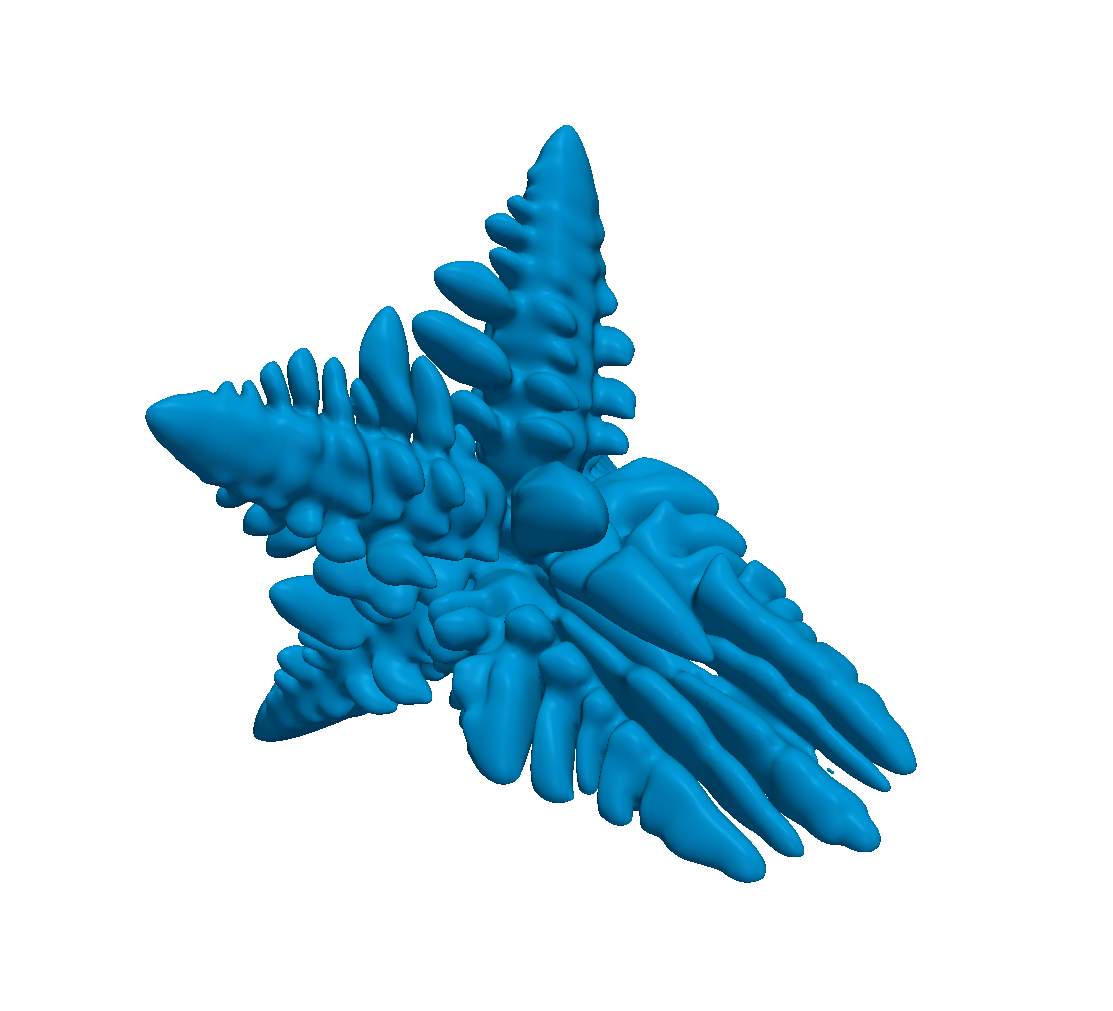
\includegraphics[width=.24\textwidth]{stefan/nb2_iter59.png}
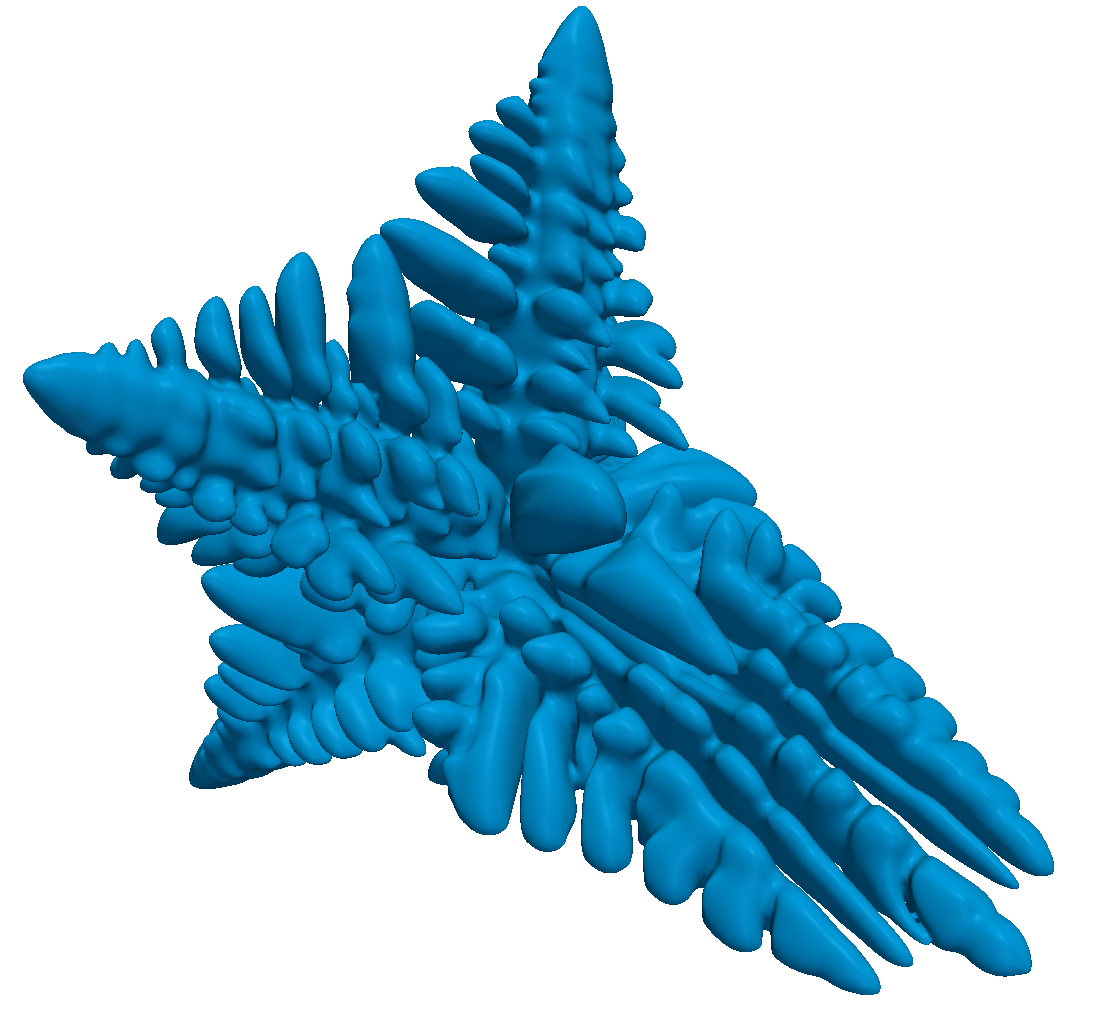
\includegraphics[width=.24\textwidth]{stefan/nb2_iter79.png}
}
\subfigure{
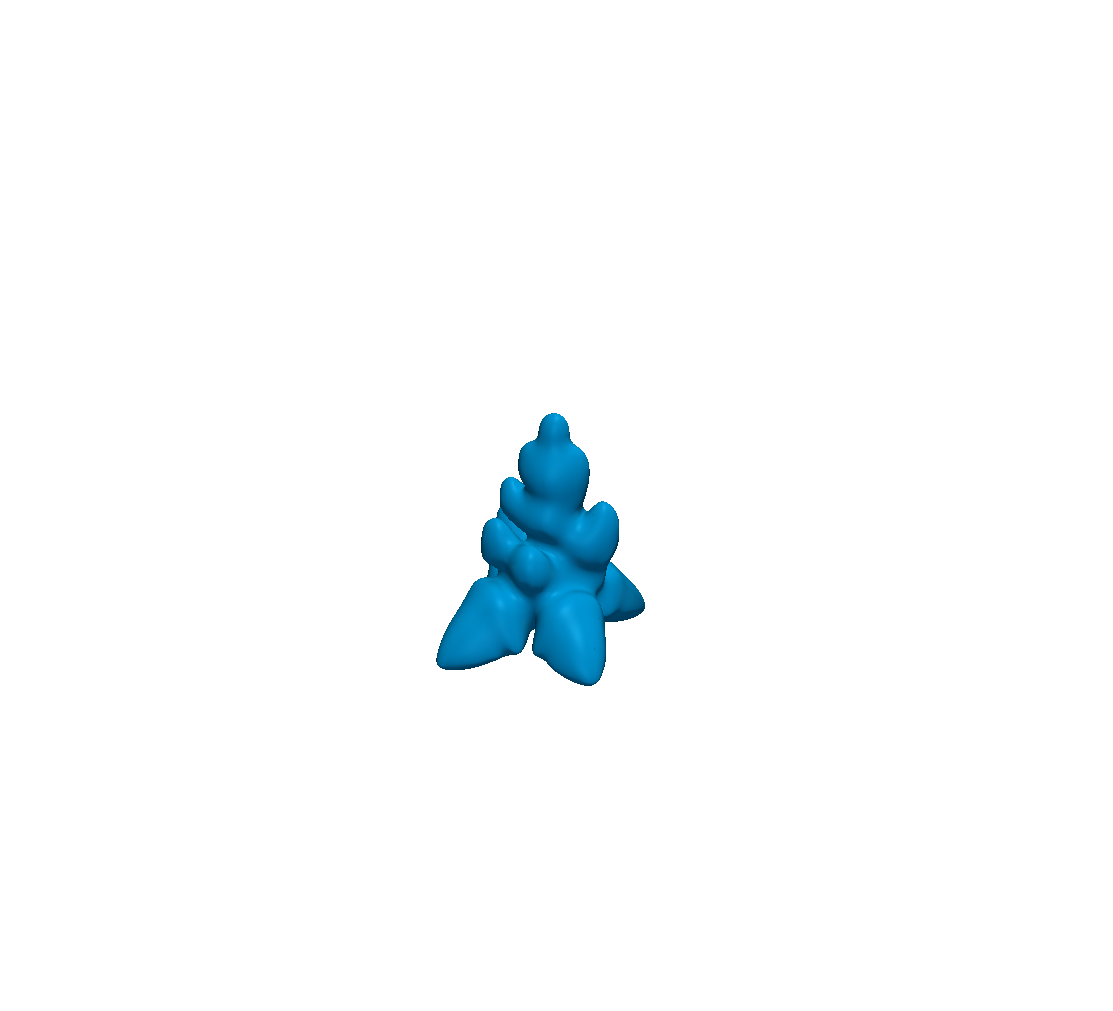
\includegraphics[width=.24\textwidth]{stefan/nb5_iter19.png}
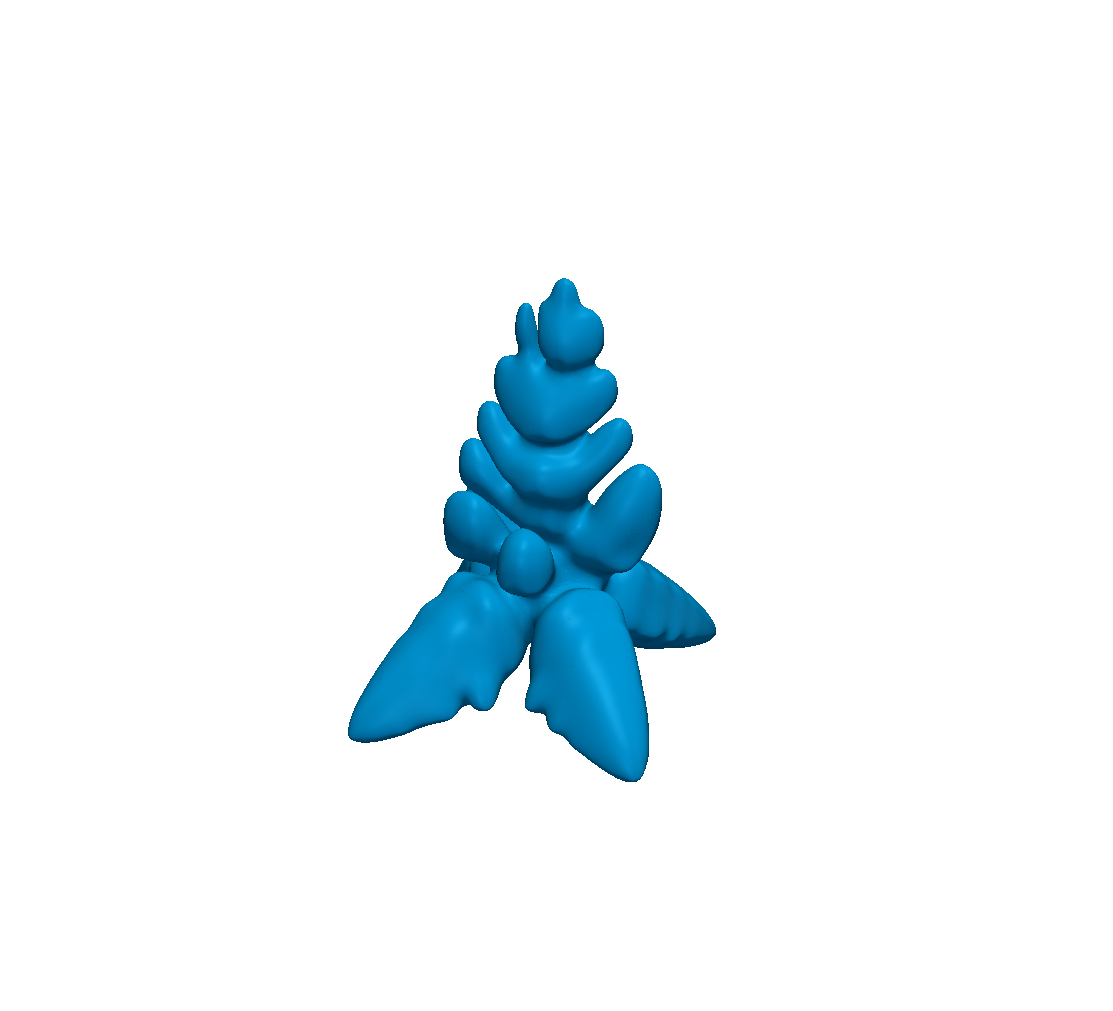
\includegraphics[width=.24\textwidth]{stefan/nb5_iter39.png}
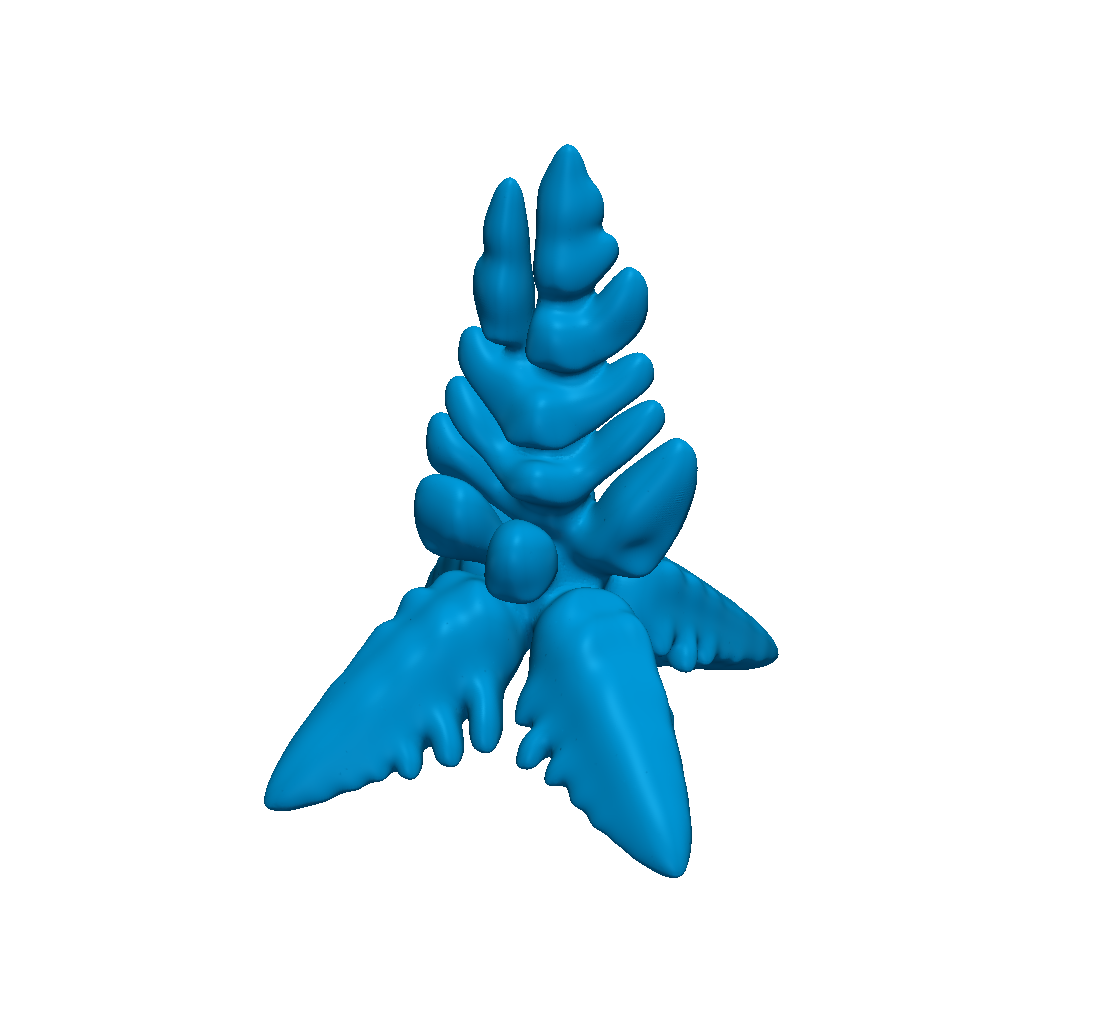
\includegraphics[width=.24\textwidth]{stefan/nb5_iter59.png}
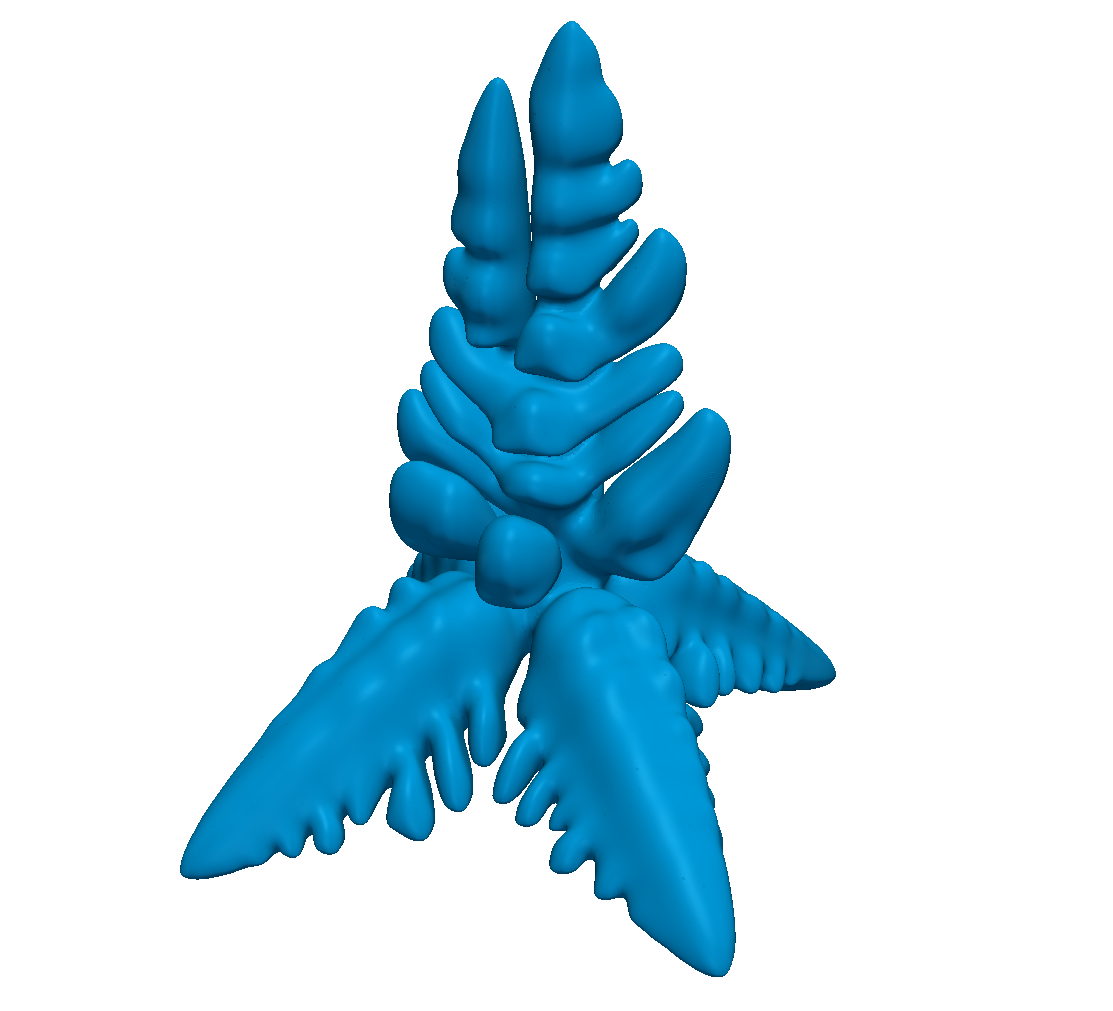
\includegraphics[width=.24\textwidth]{stefan/nb5_iter79.png}
}
\subfigure{
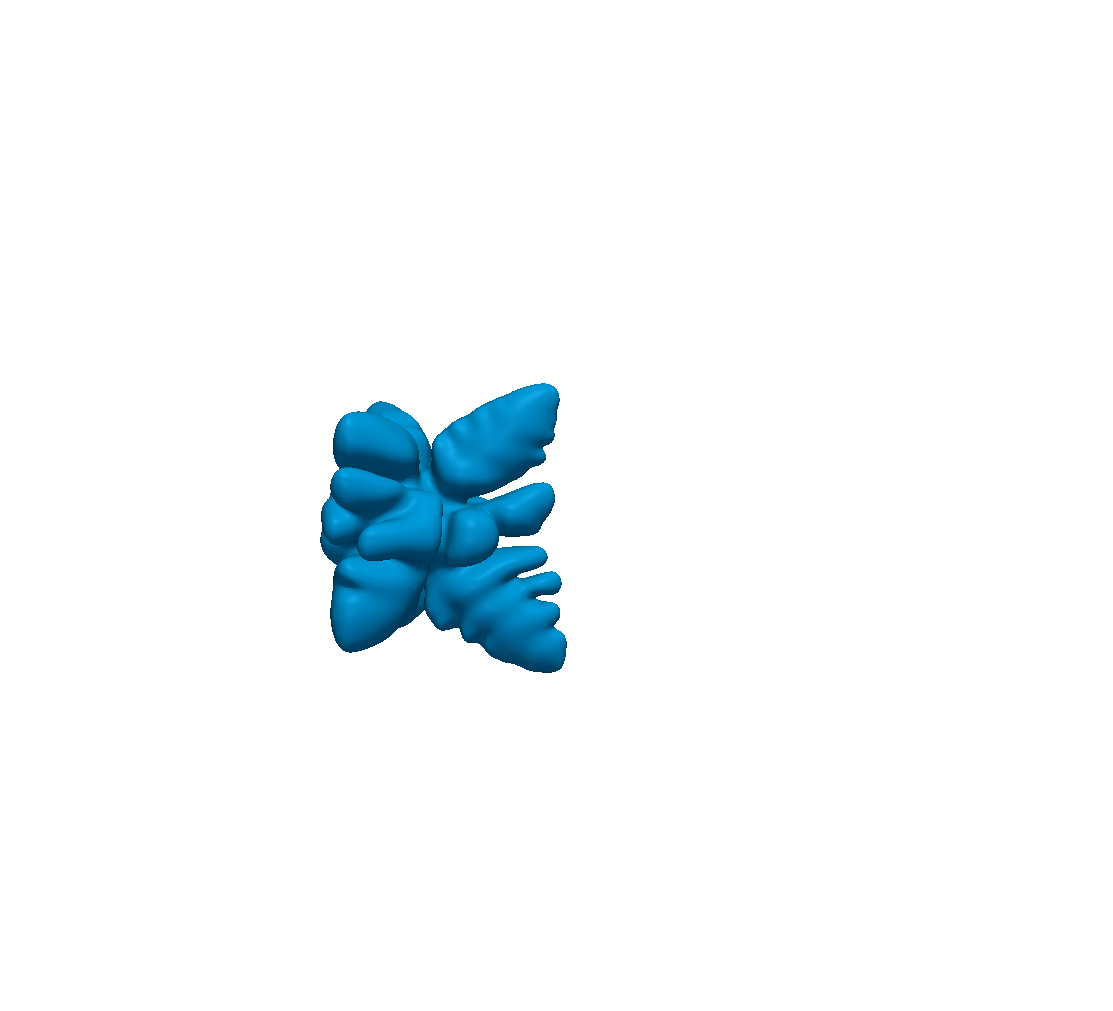
\includegraphics[width=.24\textwidth]{stefan/nb8_iter19.png}
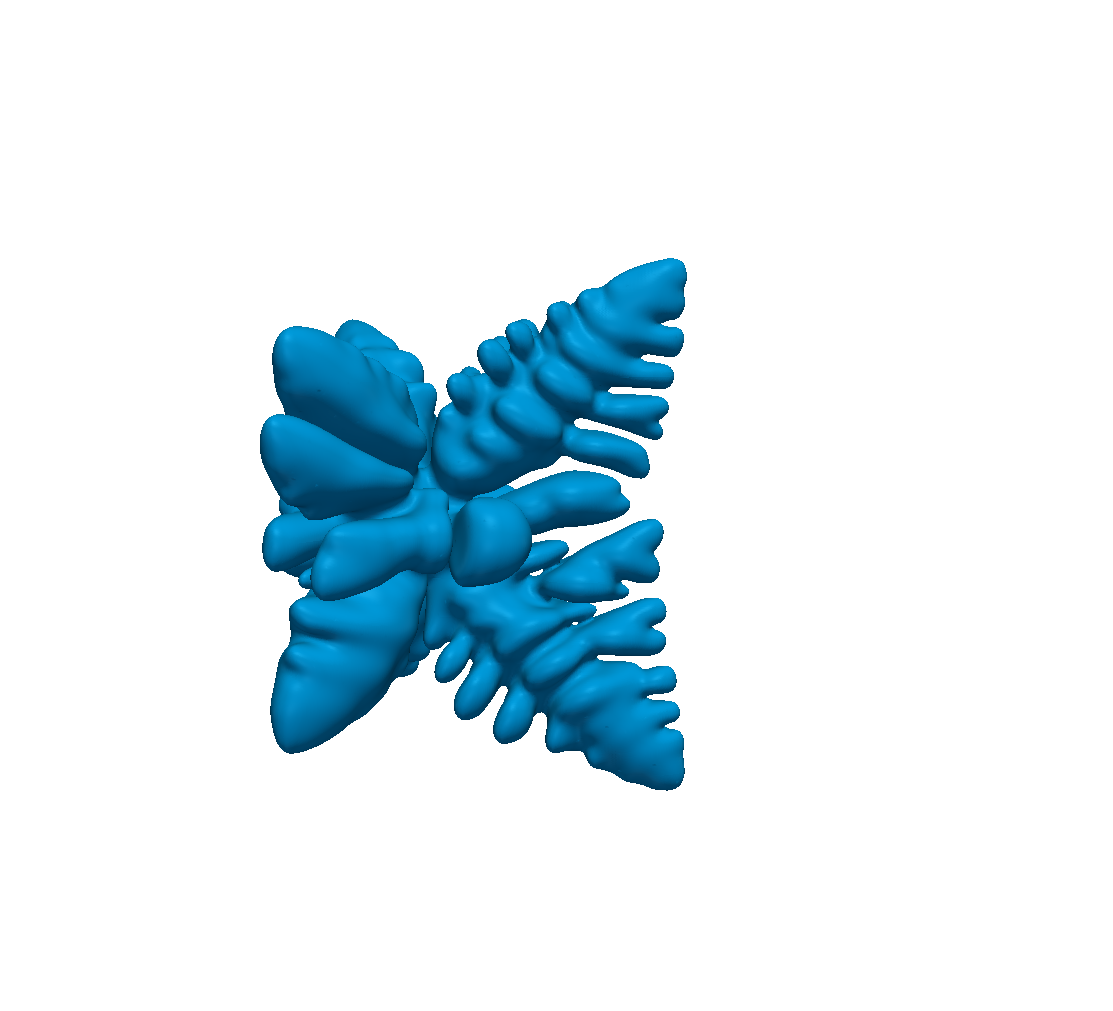
\includegraphics[width=.24\textwidth]{stefan/nb8_iter39.png}
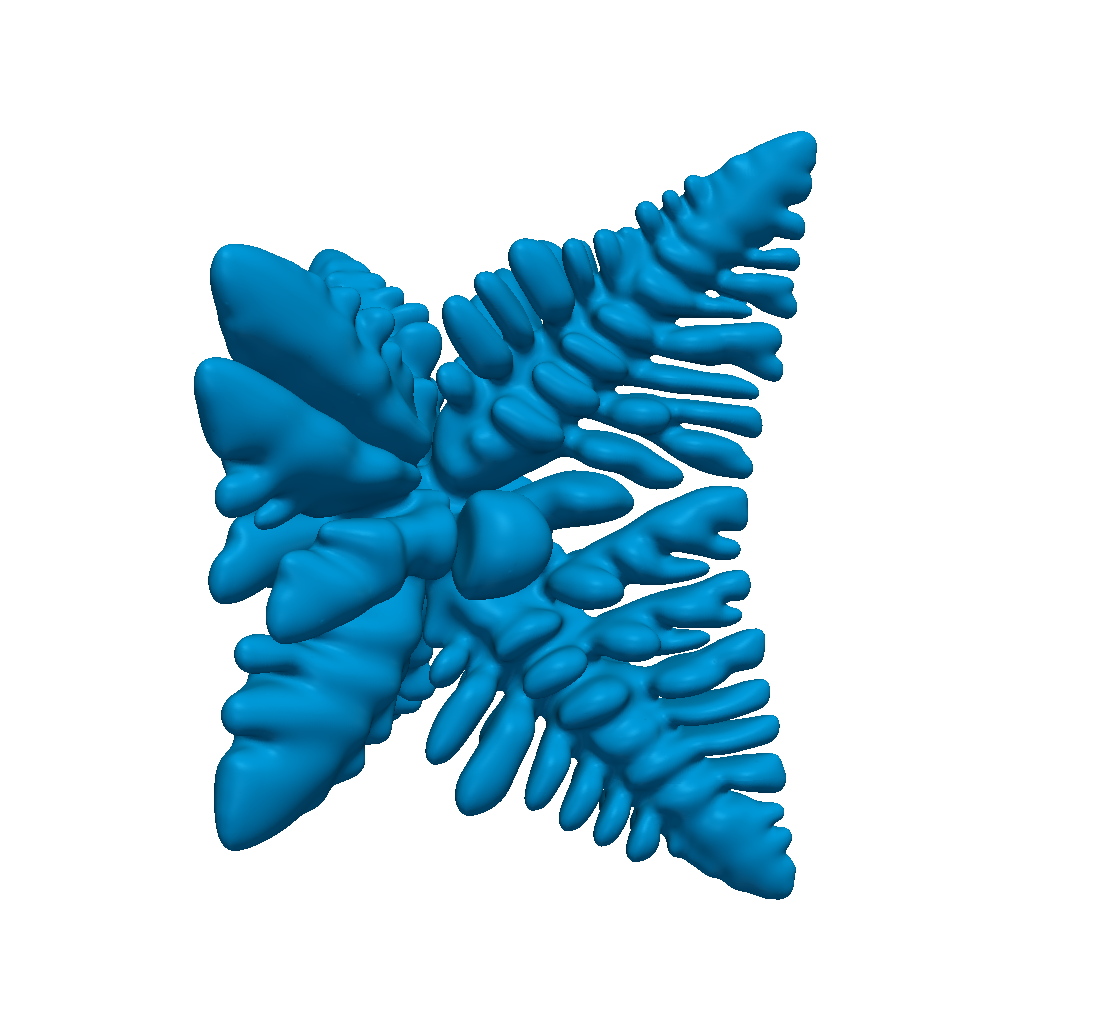
\includegraphics[width=.24\textwidth]{stefan/nb8_iter59.png}
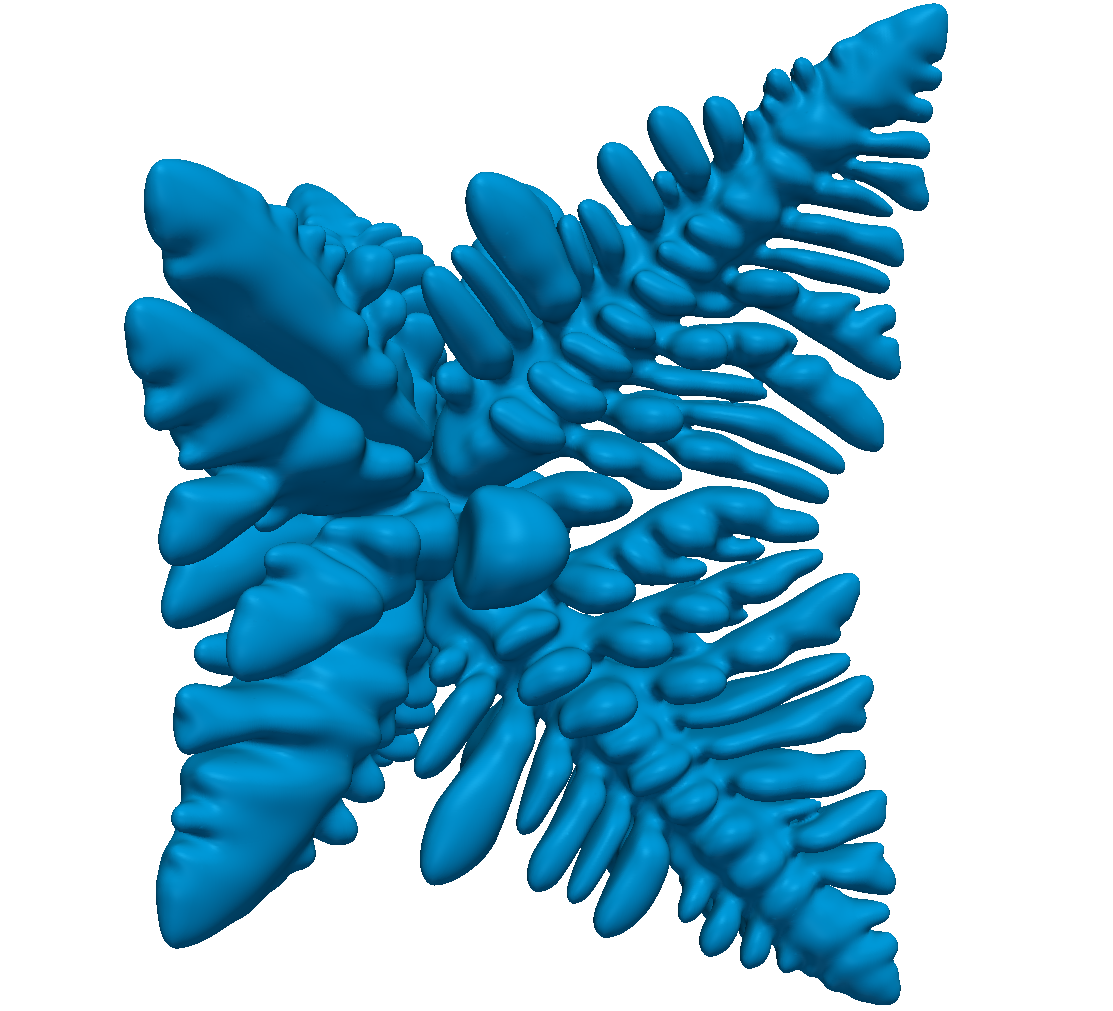
\includegraphics[width=.24\textwidth]{stefan/nb8_iter79.png}
}
\subfigure{
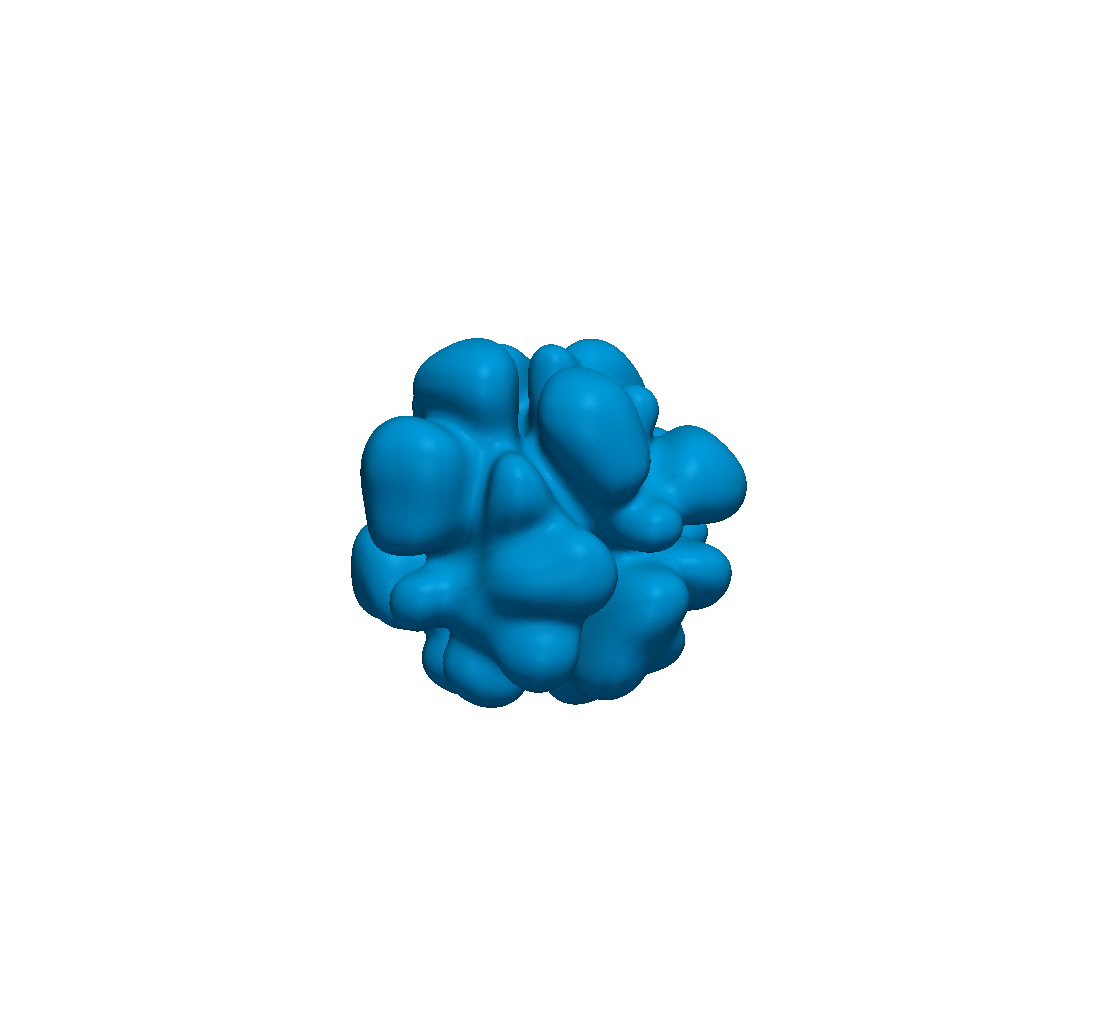
\includegraphics[width=.24\textwidth]{stefan/nb12_iter19.png}
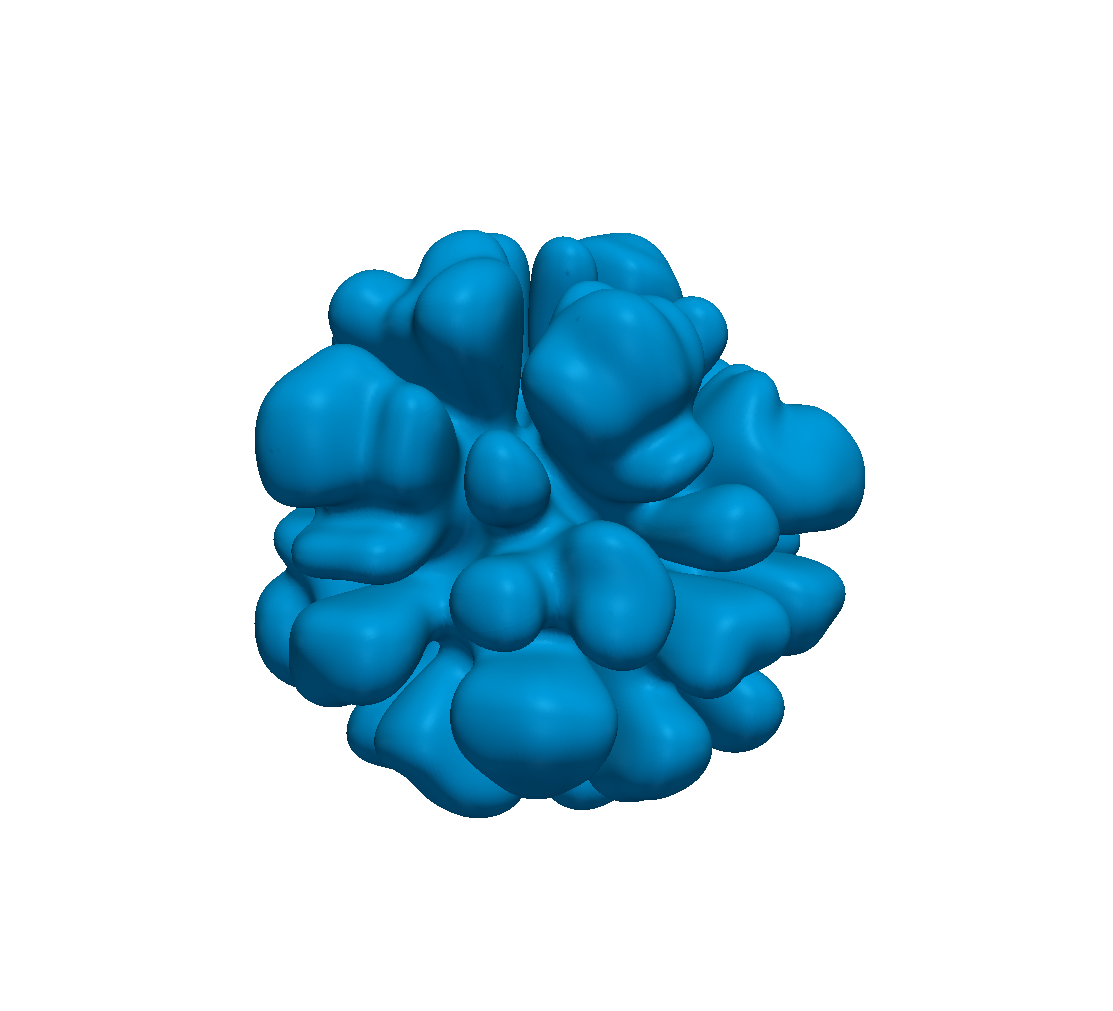
\includegraphics[width=.24\textwidth]{stefan/nb12_iter39.png}
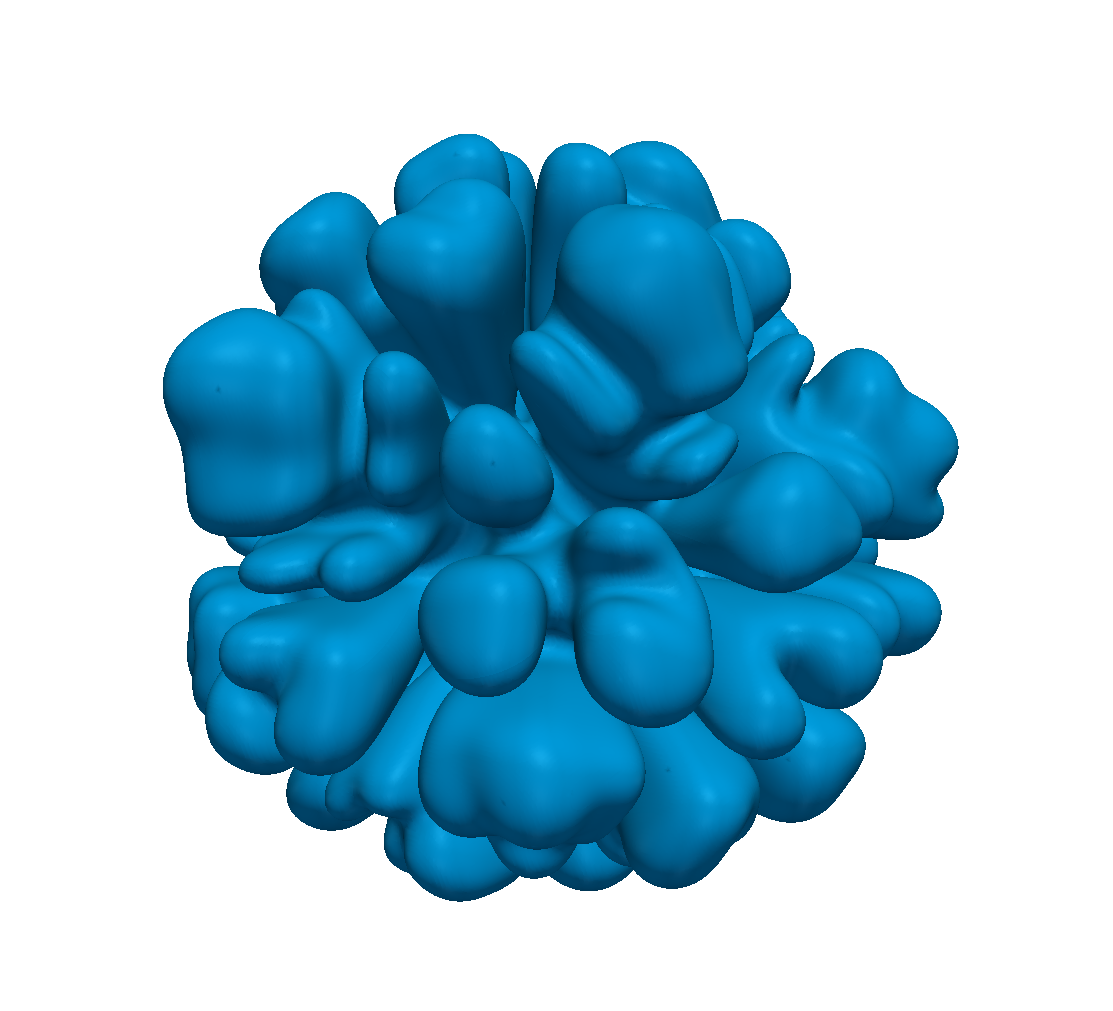
\includegraphics[width=.24\textwidth]{stefan/nb12_iter59.png}
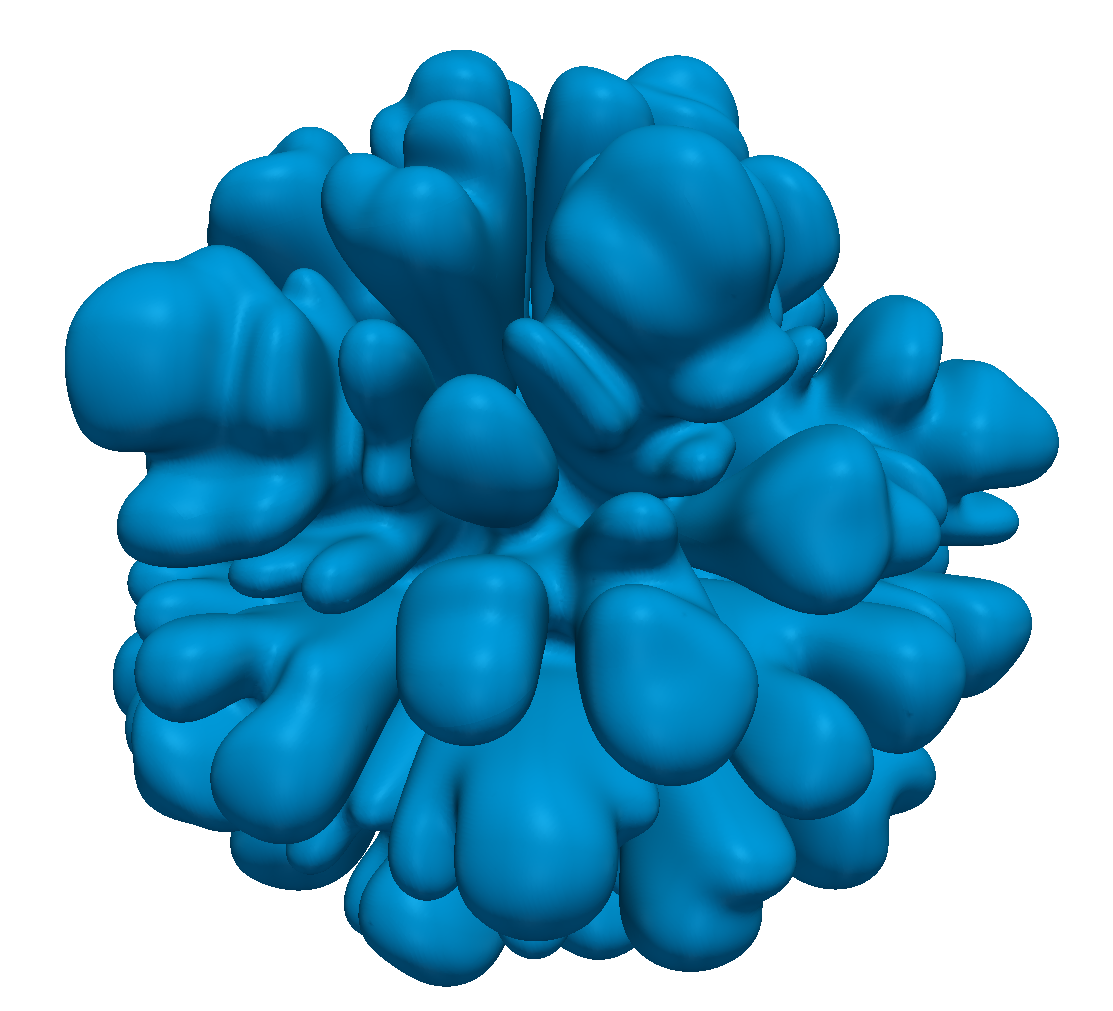
\includegraphics[width=.24\textwidth]{stefan/nb12_iter79.png}
}
\caption{Time evolution of four of the crystals obtained for the Stefan problem simulation. The snapshots represent, from left to right, iterations 96, 196, 296 and 396.} \label{fig:stefan_evolution}
\end{center}
\end{figure}
